%! TeX program = lualatex
\documentclass[12pt,a4paper]{article}

\usepackage[nil]{babel}
\usepackage{unicode-math}
\usepackage[svgnames]{xcolor}
\usepackage{lmodern}
\usepackage{graphicx}
\usepackage{wrapfig}
\usepackage{float}
\usepackage{parskip}
\usepackage{enumitem}

\makeatother
\babelprovide[import=el, main, onchar=ids fonts]{greek} % can also do import=el-polyton
\babelprovide[import, onchar=ids fonts]{english}

\babelfont{rm}
          [Language=Default]{Liberation Sans}
\babelfont[english]{rm}
          [Language=Default]{Liberation Sans}
\babelfont{sf}
          [Language=Default]{Liberation Sans}
\babelfont{tt}
          [Language=Default]{Liberation Sans}

%Enter Title Here
\title{Use-cases-v0.1 \\ LibShare}
\author{\textbf{Ονόματα / ΑΜ / Έτος:} \\ Γρηγόρης Καπαδούκας / 1072484 / 4\textdegree \\ Χρήστος Μπεστητζάνος / 1072615 / 4\textdegree \\ Νικόλαος Αυγέρης / 1067508 / 5\textdegree \\ Περικλής Κοροντζής / 1072563 / 4\textdegree}

\begin{document}

\makeatletter
\begin{center}
	\LARGE{\@title} \\
	\pagebreak
	\begin{LARGE}\@author\end{LARGE} \\
\end{center}
\pagebreak

%Insert Body Here
\section{Use Case Diagram}

Το Use Case Diagram που φτιάξαμε αποτελεί το Σχήμα \ref{Use Case Diagram}. Για την καλύτερη και πιο λεπτομερή σχεδίαση, πολλά use cases τα οποία αποτελούν ένα use case παρακάτω στο κεφάλαιο \ref{Ροές των Use Cases}, εδώ έχουν αποτελέσει περισσότερα από ένα με σκοπό την καλύτερη ανάλυση της αλληλεπίδρασης μεταξύ των use cases.

Έτσι για παράδειγμα, το use case της "Αναζήτησης βιβλίων / χρήστη, αιτήσεων" στο κεφάλαιο \ref{Ροές των Use Cases} εδώ χωρίζεται σε "Αναζήτηση", "Αναζήτηση βιβλίου", "Αναζήτηση χρήστη" και "Αναζήτηση αίτησης", με σχέση γενίκευσης των τριών τελευταίων από το πρώτο. Επίσης τα use cases με σχέση extends μπορούν στο κεφάλαιο \ref{Ροές των Use Cases} να αναπαρασταθούν σε ένα use case, με ένδειξη της επιπλέον λειτουργικότητας σε εναλλακτική ροή. Με αυτόν τον τρόπο προσπαθούμε να αποφύγουνε να αναλύσουμε τετριμμένα use cases.

\begin{figure}[H]
	\makebox[\textwidth]{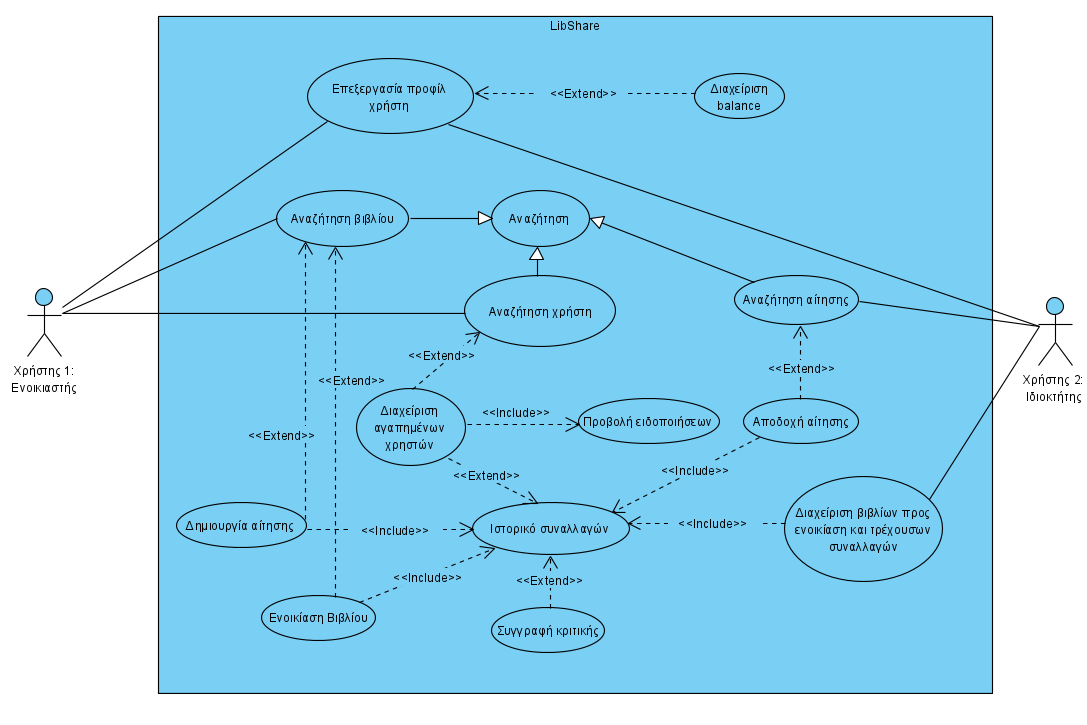
\includegraphics[width=\textwidth]{Use-case Diagram.png}}
	\caption{Use Case Diagram}
	\label{Use Case Diagram}
\end{figure}


\section{Ροές των Use Cases}
\label{Ροές των Use Cases}

\subsection{Αναζήτηση βιβλίων / χρήστη / αιτήσεων}

\subsubsection*{Βασική Ροή <<Αναζήτηση βιβλίων / χρήστη / αιτήσεων>>: Αναζήτηση βιβλίων:}
\begin{enumerate}
    \item Το σύστημα προσπαθεί να συνδεθεί στη βάση δεδομένων και το κάνει με επιτυχία.
        \label{Έλεγχος σύνδεσης στη βάση δεδομένων}
    \item Ο χρήστης επιλέγει φίλτρο αναζήτησης "βιβλία", με τύπο συναλλαγής "και τα δύο" (δηλαδή και από κοντά και ταχυδρομικώς) και εισάγει ένα κείμενο αναζήτησης (μπορεί να είναι και τίτλος βιβλίου και όνομα συγγραφέα).
        \label{Επιλογή τύπου αναζήτησης}
    \item Το σύστημα ελέγχει αν υπάρχουν διαθέσιμα βιβλία προς ενοικίαση που να πληρούν το κείμενο αναζήτησης και το τύπο συναλλαγής και βλέπει ότι υπάρχουν.
        \label{Ύπαρξη βιβλίου}
    \item Το σύστημα δείχνει τη λίστα με τα διαθέσιμα βιβλία στον χρήστη, περιέχοντας τους πλήρεις τίτλους, το όνομα συγγραφέα, τον εκδοτικό οίκο και έτος τύπωσης.
    \item Ο χρήστης επιλέγει ένα από τα βιβλία.
    \item Το σύστημα φορτώνει τη λίστα των ιδιοκτητών που προσφέρουν το βιβλίο που επιλέχθηκε και την προβάλλει στον χρήστη, μαζί με την τιμή του βιβλίου ανά μέρα, την πόλη που μένει ο κάθε χρήστης, το σκορ του (που προκύπτει από τα ratings άλλων χρηστών) και κουμπί που του επιτρέπει να κάνει αίτηση ενοικίασης του βιβλίου στον χρήστη αυτόν.
\end{enumerate}

\subsubsection*{Εναλλακτική Ροή 1: Δεν μπορεί να επιτευχθεί σύνδεση στη βάση δεδομένων:}
\begin{enumerate}
    \item[\ref{Έλεγχος σύνδεσης στη βάση δεδομένων}.1.] Το σύστημα διαπιστώνει ότι δεν μπορεί να συνδεθεί στη βάση δεδομένων.
    \item[\ref{Έλεγχος σύνδεσης στη βάση δεδομένων}.2.] Το σύστημα ενημερώνει τον χρήστη ότι η πλατφόρμα αντιμετωπίζει τεχνικές δυσκολίες.
\end{enumerate}

\subsubsection*{Εναλλακτική Ροή 2: Αναζήτηση χρήστη - Αυτός υπάρχει:}
\begin{enumerate}
    \item[\ref{Επιλογή τύπου αναζήτησης}.α.1.] Ο χρήστης επιλέγει φίλτρο αναζήτησης "χρήστης" και εισάγει ένα κείμενο αναζήτησης (το username του χρήστη που αναζητεί).
    \item[\ref{Επιλογή τύπου αναζήτησης}.α.2.] Το σύστημα ελέγχει αν υπάρχει άλλος χρήστης με το όνομα που ζήτησε ο χρήστης και βλέπει ότι υπάρχει.
    \item[\ref{Επιλογή τύπου αναζήτησης}.α.3.] Το σύστημα προβάλλει στον χρήστη το προφίλ του χρήστη που αναζήτησε, δηλαδή το username, το rating του, την τοποθεσία που μένει και το description που έχει ορίσει για τον λογαριασμό του. Επίσης προβάλλει ένα κουμπί προσθήκης χρήστη στη λίστα των αγαπημένων (το οποίο χρησιμοποιείται για το use case των notifications και αγαπημένων).
\end{enumerate}

\subsubsection*{Εναλλακτική Ροή 3: Αναζήτηση χρήστη - Αυτός δεν υπάρχει:}
\begin{enumerate}
    \item[\ref{Επιλογή τύπου αναζήτησης}.α.2.1.] Το σύστημα ελέγχει αν υπάρχει άλλος χρήστης με το όνομα που ζήτησε ο χρήστης και βλέπει ότι δεν υπάρχει.
    \item[\ref{Επιλογή τύπου αναζήτησης}.α.2.2.] Το σύστημα ενημερώνει τον χρήστη ότι ο χρήστης που αναζητεί δεν υπάρχει.
\end{enumerate}

\subsubsection*{Εναλλακτική Ροή 4: Αναζήτηση αίτησης - Αυτή υπάρχει:}
\begin{enumerate}
    \item[\ref{Επιλογή τύπου αναζήτησης}.β.1.] Ο χρήστης επιλέγει φίλτρο αναζήτησης "αιτήσεις", με τύπο συναλλαγής "και τα δύο", και εισάγει ένα κείμενο αναζήτησης (το όνομα του βιβλίου για το οποίο αναζητά αν υπάρχουν αιτήσεις).
    \item[\ref{Επιλογή τύπου αναζήτησης}.β.2.] Το σύστημα ελέγχει αν υπάρχει αίτηση που να πληρεί τα κριτήρια αναζήτησης που ζήτησε ο χρήστης και διαπιστώνει ότι υπάρχει.
    \item[\ref{Επιλογή τύπου αναζήτησης}.β.3.] Το σύστημα δείχνει τη λίστα με τα βιβλία για τα οποία υπάρχουν αιτήσεις που πληρούν τα κριτήρια αναζήτησης στον χρήστη, περιέχοντας τους πλήρεις τίτλους, το όνομα συγγραφέα, τον εκδοτικό οίκο και έτος τύπωσης.
    \item[\ref{Επιλογή τύπου αναζήτησης}.β.4.] Ο χρήστης επιλέγει ένα από τα βιβλία.
    \item[\ref{Επιλογή τύπου αναζήτησης}.β.5.] Το σύστημα φορτώνει τη λίστα των χρηστών που έχουν κάνει αίτηση για το βιβλίο που επιλέχθηκε και την προβάλλει στον χρήστη, μαζί με την τιμή που προτίθενται να πληρώσει ο κάθε χρήστης για το βιβλίο ανά μέρα, την πόλη που μένει ο καθένας, το σκορ τους και κουμπί που του επιτρέπει να κάνει αποδοχή της αίτησης.
\end{enumerate}

\subsubsection*{Εναλλακτική Ροή 5: Αναζήτηση αίτησης - Αυτή δεν υπάρχει:}
\begin{enumerate}
    \item[\ref{Επιλογή τύπου αναζήτησης}.β.2.1.] Το σύστημα ελέγχει αν υπάρχει αίτηση για το βιβλίο που αναζήτησε ο χρήστης και διαπιστώνει ότι δεν υπάρχει.
    \item[\ref{Επιλογή τύπου αναζήτησης}.β.2.2.] Το σύστημα ενημερώνει τον χρήστη ότι δεν υπάρχει αίτηση που να πληρεί τα κριτήρια αναζήτησης.
\end{enumerate}

\subsubsection*{Εναλλακτική Ροή 6: Αναζήτηση βιβλίου - Μόνο από κοντά:}
\begin{enumerate}
    \item[\ref{Επιλογή τύπου αναζήτησης}.γ.1.] Ο χρήστης επιλέγει φίλτρο αναζήτησης "βιβλία", με τύπο συναλλαγής "μόνο από κοντά" και εισάγει ένα κείμενο αναζήτησης (μπορεί να είναι και τίτλος βιβλίου και όνομα συγγραφέα).
    \item[\ref{Επιλογή τύπου αναζήτησης}.γ.2.] Η περίπτωση χρήσης συνεχίζεται από το βήμα \ref{Ύπαρξη βιβλίου} της βασικής ροής.
\end{enumerate}

\subsubsection*{Εναλλακτική Ροή 7: Αναζήτηση βιβλίου - Μόνο ταχυδρομικώς:}
\begin{enumerate}
    \item[\ref{Επιλογή τύπου αναζήτησης}.δ.1.] Ο χρήστης επιλέγει φίλτρο αναζήτησης "βιβλία", με τύπο συναλλαγής "μόνο ταχυδρομικώς" και εισάγει ένα κείμενο αναζήτησης (μπορεί να είναι και τίτλος βιβλίου και όνομα συγγραφέα).
    \item[\ref{Επιλογή τύπου αναζήτησης}.δ.2.] Η περίπτωση χρήσης συνεχίζεται από το βήμα \ref{Ύπαρξη βιβλίου} της βασικής ροής.
\end{enumerate}

\subsubsection*{Εναλλακτική Ροή 8: Αναζήτηση βιβλίου - Αυτό δεν υπάρχει:}
\begin{enumerate}
    \item[\ref{Ύπαρξη βιβλίου}.1.] Το σύστημα ελέγχει αν υπάρχουν διαθέσιμα βιβλία προς ενοικίαση που να πληρούν το κείμενο αναζήτησης και βλέπει ότι υπάρχουν.
    \item[\ref{Ύπαρξη βιβλίου}.2.] Το σύστημα ενημερώνει τον χρήστη ότι δεν υπάρχουν διαθέσιμα βιβλία που να πληρούν τα κριτήρια αναζήτησης. 
\end{enumerate}

\subsubsection*{Εναλλακτική Ροή 9: Αναζήτηση αίτησης - Μόνο από κοντά:}
\begin{enumerate}
    \item[\ref{Επιλογή τύπου αναζήτησης}.β.1.α.1.] Ο χρήστης επιλέγει φίλτρο αναζήτησης "αιτήσεις", με τύπο συναλλαγής "μόνο από κοντά", και εισάγει ένα κείμενο αναζήτησης (το όνομα του βιβλίου για το οποίο αναζητά αν υπάρχουν αιτήσεις).
    \item[\ref{Επιλογή τύπου αναζήτησης}.β.1.α.2.] Η περίπτωση χρήσης συνεχίζεται από το βήμα 2.γ.1.2 της βασικής ροής.
\end{enumerate}

\subsubsection*{Εναλλακτική Ροή 10: Αναζήτηση αίτησης - Μόνο ταχυδρομικώς:}
\begin{enumerate}
    \item[\ref{Επιλογή τύπου αναζήτησης}.β.1.β.1.] Ο χρήστης επιλέγει φίλτρο αναζήτησης "αιτήσεις", με τύπο συναλλαγής "μόνο ταχυδρομικώς", και εισάγει ένα κείμενο αναζήτησης (το όνομα του βιβλίου για το οποίο αναζητά αν υπάρχουν αιτήσεις).
    \item[\ref{Επιλογή τύπου αναζήτησης}.β.1.β.2.] Η περίπτωση χρήσης συνεχίζεται από το βήμα 2.γ.1.2 της βασικής ροής.
\end{enumerate}


\subsection{Ενοικίαση βιβλίου από άλλο χρήστη}

\subsubsection*{Βασική Ροή <<Ενοικίαση Βιβλίου>>: Συναλλαγή από κοντά:}
\begin{enumerate}
    \item Ο ενοικιαστής κάνει αίτηση ενοικίασης στον ιδιοκτήτη που επέλεξε για το βιβλίο που αναζήτησε, επιλέγοντας συναλλαγή από κοντά.
        \label{Επιλογή τρόπου συναλλαγής}
    \item Το σύστημα επιβεβαιώνει ότι ο ενοικιαστής έχει αρκετά χρήματα στο λογαριασμό του για να καλύψει το "ποσό ασφαλείας" που θα δεσμευτεί αργότερα από τον λογαριασμό του.
        \label{Έλεγχος ποσού ασφαλείας}
    \item Το σύστημα επιβεβαιώνει ότι η αίτηση ενοικίασης έχει γίνει αποδεκτή από τον ιδιοκτήτη.
        \label{Αποδοχή ή απόρριψη συναλλαγής}
    \item Το σύστημα εμφανίζει στοιχεία επικοινωνίας του ιδιοκτήτη στον ενοικιαστή.
    \item Ο ενοικιαστής, αφού βρεθεί με τον ιδιοκτήτη από κοντά και παραλάβει το βιβλίο, ενημερώνει το σύστημα ότι έχει κατοχή του βιβλίου. Ο ιδιοκτήτης επίσης ενημερώνει το σύστημα.
    \item Το σύστημα ελέγχει αν έλαβε ενημέρωση κατοχής του βιβλίου και από τον ενοικιαστή και από τον ιδιοκτήτη.
        \label {Δεν ενημερώνεται η κατοχή}
    \item Το σύστημα δεσμεύει "ποσό ασφαλείας" από τον λογαριασμό του ενοικιαστή, και αρχίζει να τον χρεώνει αυτόματα μέρα με τη μέρα.
        \label{Τέλος dispute resolved - Τέλος χρημάτων}
    \item Ο ενοικιαστής, αφού τελειώσει το βιβλίο, βρίσκεται πάλι με τον ιδιοκτήτη και του παραχωρεί το βιβλίο, έπειτα του οποίου ενημερώνουν και οι δύο το σύστημα ότι το βιβλίο έχει επιστραφεί.
        \label{Επιστροφή βιβλίου - Τέλος λεφτά δεν φτάνουν}
    \item Το σύστημα, λάβει ενημέρωση επιστροφής βιβλίου και από τα δύο μέλη, σταματάει να χρεώνει τον ενοικιαστή και του επιστρέφει το "ποσό ασφαλείας".
        \label{Τέλος ενοικίασης}
\end{enumerate}

\subsubsection*{Εναλλακτική Ροή 1: Η συναλλαγή γίνεται ταχυδρομικώς:}
\begin{enumerate}
    \item[\ref{Επιλογή τρόπου συναλλαγής}.1.] Ο ενοικιαστής κάνει αίτηση ενοικίασης στον ιδιοκτήτη που επέλεξε για το βιβλίο που αναζήτησε, επιλέγοντας συναλλαγή ταχυδρομικώς.
    \item[\ref{Επιλογή τρόπου συναλλαγής}.2.] Το σύστημα επιβεβαιώνει ότι ο ενοικιαστής έχει αρκετά χρήματα στο λογαριασμό του για να καλύψει το "ποσό ασφαλείας" που θα δεσμευτεί αργότερα από τον λογαριασμό του.
    \item[\ref{Επιλογή τρόπου συναλλαγής}.3.] Το σύστημα επιβεβαιώνει ότι η αίτηση ενοικίασης έχει γίνει αποδεκτή από τον ιδιοκτήτη και ότι έχει γίνει η αποστολή.
    \item[\ref{Επιλογή τρόπου συναλλαγής}.4.] Το σύστημα εμφανίζει τα στοιχεία του ιδιοκτήτη και tracking number από την αποστολή στον ενοικιαστή και γίνεται δέσμευση του "ποσού ασφαλείας" από τον λογαριασμό του ενοικιαστή.
    \item[\ref{Επιλογή τρόπου συναλλαγής}.5.] Ο ενοικιαστής, αφού παραλάβει το βιβλίο ταχυδρομικώς, ενημερώνει το σύστημα ότι έχει κατοχή του βιβλίου (η ενημέρωση κατοχής από τον αποστολέα γίνεται αυτόματα μέσω της κατάστασης δέματος με χρήση του tracking number).
    \item[\ref{Επιλογή τρόπου συναλλαγής}.6.] Το σύστημα, αφού λάβει ενημέρωση κατοχής του βιβλίου και από τον ιδιοκτήτη, αρχίζει να τον χρεώνει μέρα με τη μέρα.
    \item[\ref{Επιλογή τρόπου συναλλαγής}.7.] Ο ενοικιαστής, αφού τελειώσει το βιβλίο, στέλνει πίσω στον ιδιοκτήτη το βιβλίο ταχυδρομικώς και ενημερώνει τη πλατφόρμα με tracking number (το οποίο θα χρησιμοποιηθεί για να ανανεωθεί η κατάσταση κατοχής αυτόματα).
    \item[\ref{Επιλογή τρόπου συναλλαγής}.9.] Η περίπτωση χρήσης συνεχίζεται από το βήμα \ref{Τέλος ενοικίασης} της βασικής ροής.
\end{enumerate}

\subsubsection*{Εναλλακτική Ροή 2: Η συναλλαγή απορρίπτεται από τον ιδιοκτήτη:}
\begin{enumerate}
    \item[\ref{Έλεγχος ποσού ασφαλείας}\|\ref{Αποδοχή ή απόρριψη συναλλαγής}.1, \ref{Επιλογή τρόπου συναλλαγής}.2\|3.1.] Το σύστημα παρατηρεί ότι η αίτηση ενοικίασης απορρίπτεται από τον ιδιοκτήτη, ή ότι δεν έχει ο ενοικιαστής αρκετό χρηματικό ποσό στο λογαριασμό για να καλύψει το "ποσό ασφαλείας".
    \item[\ref{Έλεγχος ποσού ασφαλείας}\|\ref{Αποδοχή ή απόρριψη συναλλαγής}.2, \ref{Επιλογή τρόπου συναλλαγής}.2\|3.2.] Ο ενοικιαστής ενημερώνεται από το σύστημα ότι η αίτησή του απορρίφθηκε.
\end{enumerate}

\subsubsection*{Εναλλακτική Ροή 3: Δεν ενημερώνεται και από τους δύο η κατάσταση κατοχής - Επίλυση προβλήματος:}
\begin{enumerate}
    \item[\ref{Δεν ενημερώνεται η κατοχή}\|\ref{Επιστροφή βιβλίου - Τέλος λεφτά δεν φτάνουν}.1, 1.6.1] Το σύστημα λαμβάνει ενημέρωση κατοχής από τον ιδιοκτήτη και όχι από τον ενοικιαστή, ή αντίστροφα.
    \item[\ref{Δεν ενημερώνεται η κατοχή}\|\ref{Επιστροφή βιβλίου - Τέλος λεφτά δεν φτάνουν}.2, 1.6.2] Το σύστημα ενημερώνει και τα δύο μέλη να επικοινωνήσουν μεταξύ τους και αν δεν λυθεί το θέμα να επικοινωνήσουν με την υποστήριξη πελατών.
    \item[\ref{Δεν ενημερώνεται η κατοχή}\|\ref{Επιστροφή βιβλίου - Τέλος λεφτά δεν φτάνουν}.3, 1.6.3] Το σύστημα λαμβάνει ενημέρωση κατοχής και από τον δεύτερο χρήστη.
    \item[\ref{Δεν ενημερώνεται η κατοχή}\|\ref{Επιστροφή βιβλίου - Τέλος λεφτά δεν φτάνουν}.4, 1.6.4] Η περίπτωση χρήσης συνεχίζεται από το βήμα \ref{Τέλος dispute resolved - Τέλος χρημάτων} της βασικής ροής αν βρισκόταν στην αρχική ενοικίαση, και στο βήμα \ref{Τέλος ενοικίασης} αν βρισκόταν στην φάση επιστροφής του βιβλίου.
\end{enumerate}

\subsubsection*{Εναλλακτική Ροή 4: Δεν ενημερώνεται και από τους δύο η κατάσταση κατοχής - Επίλυση από υποστήριξη πελατών:}
\begin{enumerate}
    \item[\ref{Δεν ενημερώνεται η κατοχή}\|\ref{Επιστροφή βιβλίου - Τέλος λεφτά δεν φτάνουν}.3.1, 1.6.3.1] Το σύστημα δεν λαμβάνει ενημέρωση κατοχής και από τον δεύτερο χρήστη.
    \item[\ref{Δεν ενημερώνεται η κατοχή}\|\ref{Επιστροφή βιβλίου - Τέλος λεφτά δεν φτάνουν}.3.2, 1.6.3.2]Το σύστημα ενημερώνεται από την υποστήριξη πελατών και το "ποσό ασφαλείας" αποστέλλεται στον λογαριασμό του χρήστη που αποφάσισε η υποστήριξη πελατών ότι αδικήθηκε.
\end{enumerate}

\subsubsection*{Εναλλακτική Ροή 5: Τέλος χρημάτων ενοικιαστή - Μετέπειτα προσθήκη απαραίτητου ποσού:}
\begin{enumerate}
    \item[\ref{Τέλος dispute resolved - Τέλος χρημάτων}.1.] Το σύστημα αντιλαμβάνεται ότι έχουν τελειώσει τα χρήματα του ενοικιαστή.
    \item[\ref{Τέλος dispute resolved - Τέλος χρημάτων}.2.] Το σύστημα ζητάει από τον ενοικιαστή να προσθέσει παραπάνω χρήματα στον λογαριασμό του.
    \item[\ref{Τέλος dispute resolved - Τέλος χρημάτων}.3.] Ο ενοικιαστής προσθέτει παραπάνω χρήματα στον λογαριασμό του.
    \item[\ref{Τέλος dispute resolved - Τέλος χρημάτων}.4.] Το σύστημα αντιλαμβάνεται ότι προστέθηκαν παραπάνω χρήματα και χρεώνει από τον ενοικιαστή το ποσό που οφείλει, μαζί με 20\% επιτόκιο.
    \item[\ref{Τέλος dispute resolved - Τέλος χρημάτων}.5.] Η περίπτωση χρήσης συνεχίζεται από το βήμα \ref{Επιστροφή βιβλίου - Τέλος λεφτά δεν φτάνουν} της βασικής ροής.
\end{enumerate}

\subsubsection*{Εναλλακτική Ροή 6: Τέλος χρημάτων ενοικιαστή - Δεν προστίθεται το απαραίτητο ποσό:}
\begin{enumerate}
    \item[\ref{Τέλος dispute resolved - Τέλος χρημάτων}.3.1.] Το σύστημα αντιλαμβάνεται μετά από ένα χρονικό διάστημα ότι ο χρήστης δεν έχει προσθέσει το ποσό που οφείλει στον λογαριασμό του.
    \item[\ref{Τέλος dispute resolved - Τέλος χρημάτων}.3.2.] Το σύστημα προσφέρει αυτόματα το "ποσό ασφαλείας" στον ιδιοκτήτη και απενεργοποιεί τη δυνατότητα του ενοικιαστή να νοικιάσει άλλο βιβλίο, μέχρι να πληρώσει το χρωστούμενο ποσό.
\end{enumerate}

\end{document}
